\section{Metsandus}
Metsad omavad olulist rolli nii ühiskonna igapäevaelus kui ka planeedi heaolus.
Alates mööblis kasutatavast puidust kuni paberini, millele kirjutame. Lisaks neile
nähtavatele toodetele sisaldavad paljud ravimid, kosmeetika ja pesuvahendid
metsadest saadud kõrvalsaadusi. Rohkem kui 1,6 miljardit inimest sõltub
metsadest toidu ja kütuse saamiseks ning umbes 70 miljonit, sealhulgas paljud
põlisrahvad, peavad metsi oma koduks \cite{karsentyUnderlyingCausesRapid2003}. 
Metsad varustavad meid hapnikuga, pakuvad
varjualust, töökohti, puhast vett ja toitu, olles seega inimkonna ellujäämiseks
hädavajalikud. Kuna nii paljude inimeste elu sõltub metsadest, on metsade saatus
otseselt seotud ka meie endi tulevikuga. \cite{WWFImportanceForests} 

\section{Copernicus ja EstHub}
Copernicus on üks osa Euroopa kosmoseprogrammist (EUS), mis tegeleb planeedi jälgimisega. Copernicus programmi raames, lisaks maa pealse info kogumisele, on loodud mitmeid satelliite, mis koguvad informatsiooni kosomosest. See info on kõigile kättesaadav tasuta. Selle programmiga seotud satellite kutsutakse \textbf{Sentineliks}. \cite{CopernicusCopernicus}

EstHub on Eesti riiklik satelliitandmete keskus, mis kogub ja integreerib
mitmekesiseid georuumilisi andmeid automatiseeritud protsesside kaudu.
Andmekogumine hõlmab kõrge resolutsiooniga satelliitkaadrite allalaadimist ja
standardiseerimist erinevatest allikatest. EstHubi eesmärk on koguda kokku sateliidi andmed mis katavad Eesti territooriumi. \cite{maa-ametNationalSatelliteData}

\begin{figure}[hb] % h-here, if possible; H-here, definitely; t-top of the page; b-bottom of the page; p-page of floats
    \centering
    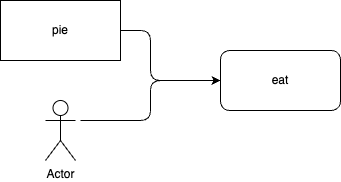
\includegraphics[width=.5\textwidth]{figures/test.drawio.png} % Includes an image from the specified path, setting the width to 50% of the text width
    \caption{An image of me enjoying a pie..} % Provides a caption for the figure, italicizing the text
    \label{fig:testpie} % Sets a label for the figure to be referenced later
\end{figure}


\subsection{Sentinel}
Sentinel-1 on radaripõhine satelliit, mis võimaldab jälgida maapinna vajumist,
struktuuride kahjustusi ning geohazarde nagu maavärinad ja maalihked. Samuti on
see ideaalne mere- ja Arktika seireks, sealhulgas laevade jälgimiseks ning
naftareostuse tuvastamiseks. \cite{S1Applications}

Sentinel-2 missioon koosneb kahest identsest satelliidist, Sentinel-2B
(käivitatud 2017) ja Sentinel-2C (käivitatud 2024), mis töötavad koos, et
pakkuda kõrge eraldusvõimega multispektraalseid pilte Maa pindadest,
rannikualadest ja siseveekogudest iga viie päeva järel. Need andmed toetavad
rakendusi põllumajanduses, metsanduses ja maakatte klassifitseerimisel. \cite{S2Applications}

Sentinel-3 on Euroopa Maa seire satelliitmissioon, mille eesmärk on mõõta
merepinna topograafiat, mere ja maa pinnatemperatuure ning ookeani ja maa
pinnavärvi suure täpsusega. Neid andmeid kasutatakse ookeani prognoosisüsteemides,
keskkonnaseires ja kliimaseires. \cite{S3Mission}

Sentinel-5P on esimene Copernicuse missioon, mis on pühendatud atmosfääri
seirele. See kannab tipptasemel \textbf{Tropomi} instrumenti, mis kaardistab mitmeid
gaase nagu lämmastikdioksiid, osoon, formaldehüüd, vääveldioksiid, metaan,
vingugaas ja aerosoolid - kõik need mõjutavad meie hingatavat õhku, tervist ja
kliimat. \cite{S5PApplications}
\subsection{Lainepikkuste spekter}

\section{Masinõppe meetodite kasutus kaugseires}